\section*{Exercice 125 -- TEC -- Clever INFOS MANQUANTES  ?}
\setcounter{exo}{0}
%Banque PT SI A 2013


\subsection*{Première correction}
Afin de répondre au critère du cahier des charges concernant la précision statique du système, on choisit de placer un intégrateur comme premier correcteur : $H_r(p)=\dfrac{K_i}{p}$.

% QUESTION 40
\subparagraph{}
\textit{On donne sur le Cahier Réponses le diagramme de Bode de la fonction de transfert en boucle ouverte $ \text{FTBO}_2(p)$ du système asservi pour $K_i = 1$ et telle que $M(p) = \text{FTBO}_2(p).\varepsilon(p)$. Déterminer, en expliquant clairement la méthode employée, la valeur de $K_i$ qui permet d'obtenir la dynamique souhaitée.}
\ifprof
\begin{corrige}
\end{corrige}
\else
\fi

On donne en annexe page 8 la définition d'un correcteur à avance de phase.
% QUESTION 41
\subparagraph{}
\textit{Combien de correcteurs à avance de phase réglés pour apporter chacun 50\degres au maximum faudrait-il incorporer dans le régulateur pour satisfaire le critère de marge de phase du cahier des charges ?}
\ifprof
\begin{corrige}
\end{corrige}
\else
\fi



On souhaite réaliser une simulation du comportement temporel du système ainsi corrigé pour un passage de 0 à 45\degres de l'habitacle en \SI{0,75}{s}. Le signal de consigne est donné sur la Figure \autoref{fig_3_2}. Le logiciel de simulation ne possède pas de bloc de signal d'entrée correspondant à ce type de fonction, mais il est possible d'utiliser des blocs de type  <<~rampe~>> possédant les critères :
\begin{itemize}
\item pente de la rampe ;
\item instant de départ de la rampe.
\end{itemize}


\begin{figure}[H]
\centering
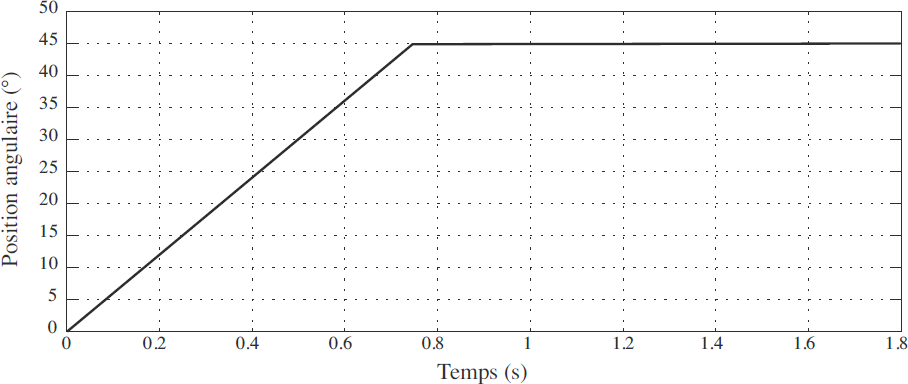
\includegraphics[width=\linewidth]{fig_3_2}
\caption{ Signal de consigne pour une simulation d'une rotation de 0 à 45\degres en \SI{0,75}{s}}
\label{fig_3_2}
\end{figure}


\subparagraph{}
\textit{Donner les paramètres à entrer dans les 2 blocs de type << rampes >> et préciser l'opération mathématique à effectuer entre les deux blocs afin d'obtenir le signal présenté sur la \autoref{fig_3_2}.}
\ifprof
\begin{corrige}
\end{corrige}
\else
\fi

La réponse obtenue par la simulation est présentée sur la \autoref{fig_3_3}.

\subparagraph{}
\textit{Quels sont les critères non satisfaits ?}
\ifprof
\begin{corrige}
\end{corrige}
\else
\fi


\begin{figure}[H]
\centering
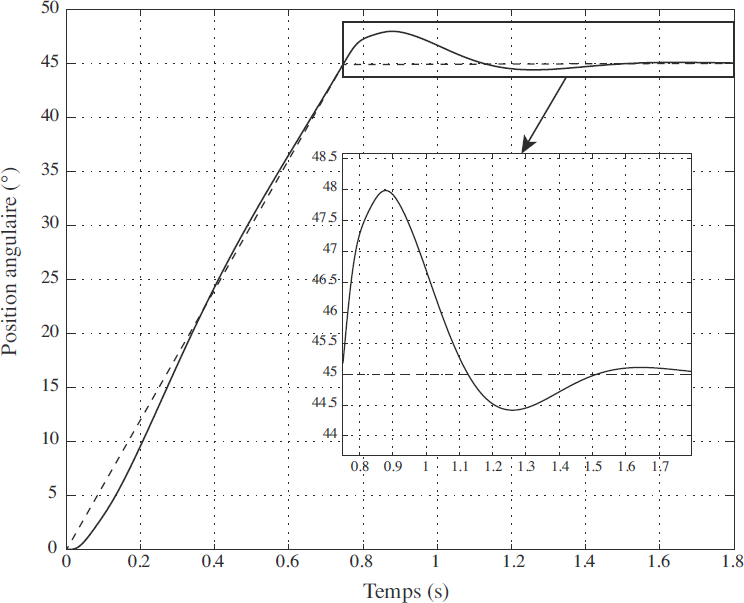
\includegraphics[width=\linewidth]{fig_3_3}
\caption{Résultat de la simulation du passage de de 0 à 45\degres en \SI{0,75}{s}}
\label{fig_3_3}
\end{figure}




\subsection*{Deuxième correction}

Plusieurs réglages du correcteur précédent ont été réalisés mais aucun n'a pu apporter satisfaction quant aux différents critères du cahier des charges. Le problème de fond ici est lié au fait que la pulsation de coupure $\omega_V$ du mode de second ordre de la fonction de transfert du vérin est inférieure à la pulsation à \SI{0}{dB} souhaitée pour garantir une dynamique suffisante du système bouclé. On souhaite donc augmenter la valeur de la pulsation de coupure $\omega_V$ afin de garantir au moins deux décades d'écart avec la pulsation à 0 dB de la fonction de transfert en boucle ouverte du système.

\subparagraph{}
\textit{Quelle valeur de diamètre du vérin permet de vérifier la condition précédente. Cette valeur est-elle réaliste ?}
\ifprof
\begin{corrige}
\end{corrige}
\else
\fi


On décide alors de remédier à ce problème par un filtre électronique du second ordre de type Notch 
de fonction de transfert :
$H_{N}(p)=\dfrac{1+ \dfrac{2\xi_n}{\omega_n}p + \dfrac{p^2}{\omega_n^2} }{1+ \dfrac{2\xi_d}{\omega_d}p + \dfrac{p^2}{\omega_d^2} }$.

Le réglage optimum du correcteur doit compenser parfaitement le mode de second ordre de la fonction de transfert du vérin. Pour cela, on effectue un essai afin d'identifier les caractéristiques de ce mode. Aucun réglage spécifique du débit de fuite n'a été réalisé, la compensation du mode rendant inutile cette étape.

Une tension de consigne $u_e(t) = 0,02u(t)$ (avec $u(t)$ l'échelon unitaire) est envoyée en entrée du servo-distributeur. Une génératrice tachymétrique, dont le comportement est modélisé par un gain pur $K_{\text{gt}} = \SI{2}{V.rad^{-1}.s}$, mesure la vitesse de rotation de l'habitacle. Cette tension est notée $m_{\omega}(t)$. Le résultat de cet essai est donné sur la Figure de la question 24 du Cahier Réponses.


\subparagraph{}
\textit{Compléter sur le Cahier Réponses le schéma-blocs représentant cet essai et déterminer la fonction de transfert $H_{\text{essai}}$ telle que : $M_{\Omega}(p) = H_{\text{essai}}(p)U_e(p)$.}
\ifprof
\begin{corrige}
\end{corrige}
\else
\fi


 
\subparagraph{}
\textit{En vous aidant du graphe de la Figure \autoref{fig_3_4}, déterminer les valeurs numériques expérimentales de $\omega_v$ et 
$\xi_v$ à partir de la courbe obtenue expérimentalement tracée sur le Cahier Réponses.}
\ifprof
\begin{corrige}
\end{corrige}
\else
\fi

\subparagraph{}
\textit{Quels inconvénients sur le comportement réel du système peuvent découler de cette méthode consistant à vouloir compenser le mode de second ordre de la fonction de transfert du vérin par ce type de filtre électronique ?}
\ifprof
\begin{corrige}
\end{corrige}
\else
\fi


\begin{figure}[H]
\centering
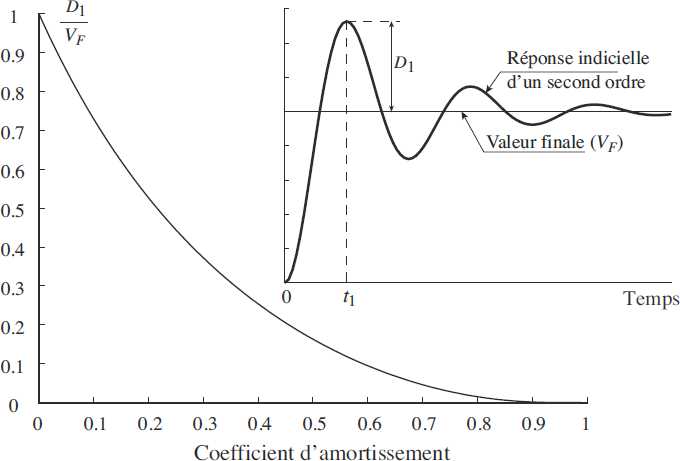
\includegraphics[width=\linewidth]{fig_3_4}
\caption{Évolution du premier dépassement relatif à la valeur finale en fonction du coefficient d'amortissement (pour une fonction de transfert du second ordre)}
\label{fig_3_4}
\end{figure}


On suppose par la suite que le numérateur du filtre Notch compense parfaitement le mode de second ordre de la fonction de transfert du vérin. On adopte les caractéristiques suivantes pour le dénominateur :
\begin{itemize}
\item $\omega_d = \SI{1000}{rad.s^{-1}}$ ;
\item $\xi_d = 1$.
\end{itemize}

Afin de satisfaire le critère de précision statique du cahier des charges on place un premier correcteur de type intégrateur non unitaire de fonction de transfert :
$H_{\text{cor2}}(p)=\dfrac{K_{\Omega}}{p}$.

La valeur de $K_{\Omega}$ est déterminée afin d'obtenir une pulsation à \SI{0}{dB} de la fonction de transfert en boucle ouverte de \SI{65}{rad.s^{-1}}. Le diagramme de Bode de cette fonction de transfert est donné sur la Figure III.5.
On complète le régulateur par un correcteur à avance de phase de fonction de transfert :
$H_{\text{av}}(p)=K_{\text{av}}\dfrac{1+a_{\text{av}}\tau_{\text{av}}p}{1+\tau_{\text{av}}p}$ avec $a_{\text{av}}>1$.

On donne en annexe page 8 la définition d'un correcteur à avance de phase.

\subparagraph{}
\textit{Déterminer les valeurs approximatives des paramètres $a_{\text{av}}$, $\tau_{\text{av}}$ et $K_{\text{av}}$ qui permettent de satisfaire le critère de marge de phase du cahier des charges tout en conservant une pulsation à \SI{0}{dB} de \SI{65}{rad.s^{-1}}.}
\ifprof
\begin{corrige}
\end{corrige}
\else
\fi



Le régulateur étant a priori optimisé, on réalise un essai de validation du comportement temporel de l'inclinaison de l'habitacle, le véhicule étant à l'arrêt. Le calculateur envoie un signal de consigne représentant l'évolution de la position angulaire souhaitée (de 0 à 45\degres en \SI{0,75}{s}). La tension délivrée par le capteur angulaire est récupérée par un convertisseur analogique-numérique afin de tracer sur un ordinateur l'évolution temporelle de l'inclinaison de l'habitacle mesurée en degrés. Les deux courbes sont données sur la \autoref{fig_3_6}.


\subparagraph{}
\textit{Quels sont les critères du cahier des charges validés ?}



\begin{figure}[H]
\centering
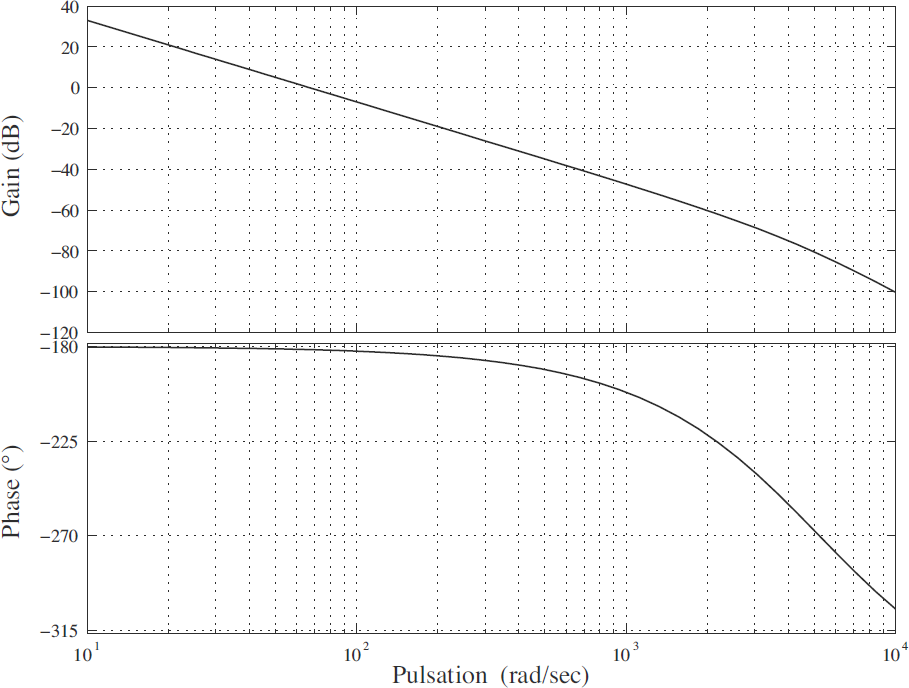
\includegraphics[width=\linewidth]{fig_3_5}
\caption{Diagramme de Bode de la Fonction de Transfert en Boucle Ouverte après correction Intégrale}
\label{fig_3_5}
\end{figure}



\begin{figure}[H]
\centering
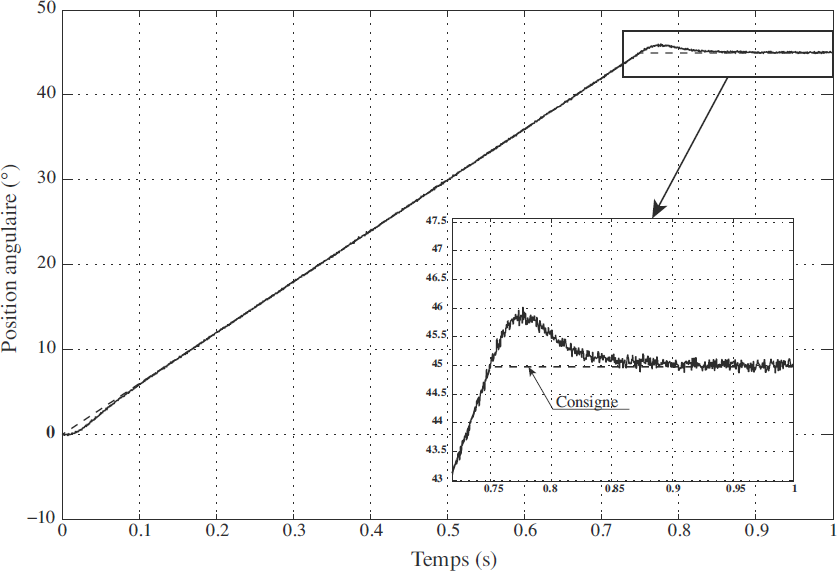
\includegraphics[width=\linewidth]{fig_3_6}
\caption{ Essai de validation : passage de 0 à 45\degres \, en  \SI{0,75}{s}}
\label{fig_3_6}
\end{figure}

